\documentclass{article} 

\usepackage{graphicx}
\usepackage[utf8]{inputenc}
\usepackage[nottoc]{tocbibind}

\begin{document} 

\title{Project plan}
\author{Ronald Kluft \and Bram Nieuwenhuize \and Boris Arkenaar}
\date{\today}
\maketitle 
\tableofcontents

\section{Introduction} 
% Geef een korte toelichting op de achtergronden van het 
%projectplan: 
% Wat ging eraan vooraf? Welke stappen zijn genomen? 
% Geef vervolgens een toelichting op de opbouw van het projectplan als 
% leeswijzer. Per hoofdstuk geeft u in één of twee zinnen aan wat er in dat 
% betreffende hoofdstuk staat. Tot slot geeft u in de inleiding een voorstel 
% tot uitvoering aan. Dat wil zeggen: Wanneer denkt men te starten met de 
%uitvoering van het project? Indien er tijd zit tussen de afronding van het 
%projectplan en de start van het project, wat wordt er in de tussentijd gedaan? 

In chapter 2 we explain the background of this project is to be found in the 
search for a way to improve JavaScript education. We see a good example of how 
JavaScript is being educated at the OU. Chapter 3 states that the objective of 
the project is to create a Program to automatically check program code 
constructed of JavaScript. In the near future we, or another team, might be 
looking at checking a combination of JavaScript and HTML. In Chapter 4 we 
explain that for realizing this project we will start off with the individual 
domain research to find out in what direction it would be best to proceed with 
the project. Chapter 5 explains the structure of the project and the 
stakeholders. 

\section{Initial Situation} 
% Bram 
% Beantwoord de vragen: 
% Waarom wil de opdrachtgever dit project? 
% Wat is de huidige situatie? 

The background of this project is to be found in the search for a way to
improve JavaScript education, whereby distance education is the dominant
form. This form should be kept in mind, for it changes the set of educational
instruments, being held against a traditional form like classroom
education. For example, the amount of interaction between teacher and student
and students among each other is no major aspect of distance education. This
complicates the possibility to provide accurate feedback. It may be argued this
problem transcends distance education, as being a general problem of mass
education in general. This might be true, and only strengthens the importance
of this project, accounting that receiving feedback is a crucial aspect of
acquiring certain skills and knowledge.

Learning a programming language like JavaScript is not a straightforward
process. Programming in general has many facets, there are many different
styles and ways to perform this art. Provided with some basic techniques, a few
syntax rules and a method for running a written program, it's quite easy for a
student to get some feedback, even on the particular written elaborations of
exercises: the written code executes (with (un)expected result), or it produces
some kind of error. Is this kind feedback useful? Is it sufficient?

\subsection{Feedback in the current situation} 
% Welke problemen en oorzaken zijn de aanleiding geweest tot de wens om te 
% veranderen? 
% Hoe ziet de omgeving eruit? Beschrijf deze vanuit het oogpunt van de 
% opdrachtgever. 

The course 'Web applications: The Client
Side'\footnote{http://www.ou.nl/studieaanbod/T58221} (developed and distributed
by the Open University) is a good example of how JavaScript is being educated
at the Open University. A student is being provided with some theoretical
material, and a set of exercises and corresponding 'proper' solutions. In the
current situation, students elaborate a given exercise. To check whether the
result is adequate, they can validate it with the provided answer, and/or
submit it for review by the professor. Both options have some shortcomings: in
programming there are often multiple good solutions for a problem, so it’s not
unlikely the elaborated answer is fundamentally different from the provided
one. In these cases the provided answer has no value in terms of giving
feedback. Submitting the answer for review overcomes this problem, but leads to
a time and labor-intensive task for the professor. In order to keep it
manageable, the professor scans the submitted answers to select common errors
and difficulties, and then provide some feedback on this selection. This
requires students to translate this generalization back to their own answer,
just like what happens in comparison a specific answer with the provided
answer.

Returning to the question whether the feedback gained by executing code is 
valuable. The description of the current situation does not explicitly answers 
the question, though the alternative (provide a proper (one of the often 
many) solution or manual reviewing by a professor) methods to generate
feedback suggests that the execution of code is not sufficient. 
Solving a problem by writing a JavaScript program is a creative process, 
with often a multitude of more or less correct solutions. Because of 
this variation in solutions, just succesfully terminating the code does 
not suffice to ensure a student has written a proper solution. 
The currently used alternative techniques both have some serious flaws. 

Another subject should be taken in mind as well. The Open University has
adopted an educational model that goes by the name of Activation Education. An
important aspect in this model is learning by doing, where the student is
encouraged to take the freedom of using the own creativity and decisiveness in
order to solve a problem. This stresses the use of {\em proper} solutions, in
the sense working towards that specific solution will not contribute to the
intended education style. Reviewing solutions for problems that encourages
creativity and decisiveness are likely harder to interpret and compare in a
search for common errors, resulting in an even bigger workload for the
professor. This should be kept in mind when developing. Even if its a bridge
too far to realize support for these kind of problems within this project, it
might be useful to create a foundation that's able to serve for this purpose in
a later stage.

\subsection{Initial Documentation}
% Welke documentatie ligt ten grondslag aan het project? 
% Welke kwaliteiten heeft deze documentatie? 
% Welke activiteiten moeten er nog verricht worden om deze documentatie te 
% complementeren? 

Harry Passier, initiator and primary stakeholder of this project, provided us 
with some guidance in the form of literature, academic papers and working 
groups. These might be of use during this project. A significant part of the 
first parts of the next phase will be used to explore the contents of these 
artifacts:
\begin{itemize}
  \item Parts of PHD initiator, namely: Chapter 1.2 until page 36, figure 2.2
    (conditions of possibility to provide feedback), Epiloque (classification),
    Page 139.
  \item {\em Ideas}\footnote{http://ideas.cs.uu.nl/} (Bastiaan Heeren, Alex
    Gerdes).
  \item {\em Web applications: the Client Side}, course material of the course
    of the {\em Open University}.
  \item {\em Software Evolution}, course about programming quality and
    indicators of good code.
\end{itemize}

\section{Project result}
% Ronald 
% % Geef antwoord op de vraag: 
% Wat is het uieindelijke resultaat van het project? 

\subsection{Objective}
 % Wat is het achterliggende doel van de opdrachtgever? 
% Wat is de koppeling tussen bedrijfsprocessen en de omgeving, gezien door de 
% bril van de opdrachtgever? 

The objective of the project is to create a Program to automatically check
solutions constructed of JavaScript code, initially the submitted code from
students of the course {\em Web applications: the Client Side}. this to reduce
the amount of time spentby the Professors to correct the solutions to exercises
and giving useful and constructive feedback to enhance didactical value in
general, and JavaScript knowledge and skills in particular, to the student. The
program should be developed in such a way it can be easily extended, modified
and reused. A thinkable extension might be the evaluation not only of
JavaScript code but of a combination with HTML as well.

\subsection{Result} 
% Wat is aan het einde van het project het concrete resultaat? 

The goal is to provide a functioning program that is able to examine and 
generate feedback on JavaScript code. The examination will be based on: 

\begin{itemize} \item Domain knowledge about syntactical and semantical
constructions possible in JavaScript; \item Input from the professor, namely an
information set containing all required information of a specific
problem/exercise; \item Input from the student, namely the solution for the
specific problem/exercise. \end{itemize} To make this possible, a tutor should
be able to add or create an exersize. A student must be able to submit a
solution for review. The result should complement to the course Webapplication:
the clientside, in particular chapter 4-7.

\subsection{Quality} 
% Wat zijn de kwaliteitseisen die gesteld worden aan het eindresultaat? 

The specific quality requirements are to be specified at the start of the
development, based on the developmental and architectual decisions. In general,
the primary aim is to create a well designed and properly functioning program,
even if this leads to a limited set of features and functions. Quality over
quantity is an important motto for the project.

\subsection{Assignment} 
% Wat is de projectopdracht in precieze bewoordingen? 
% Wat wordt wel en wat wordt niet gerekend tot de opdracht? 
% Wat zijn de eisen en beperkingen die de opdrachtgever stelt aan tijd, geld, 
% mensen of middelen?
% Wie is de opdrachtgever en wat zal hij bijdragen aan het realiseren van de 
% opdracht? 

The project assignment: "Realiseer een programma voor het automatisch nakijken 
van JavaScript en HTML." The included tasks are (in no particular order): 

\begin{itemize}
  \item Analyze a user context
  \item Architecture of a (technical) solution
  \item Designing a Program
  \item Building a Program
  \item Implementing a Program
  \item Literature study
\end{itemize}

The project owner is Dr. ir. Harrie Passier. He will contribute by giving
feedback, asking constructive questions, make go/no-go decissions and checking
the work allready done. There is a time constraint. The amount of time that can
be spent on the project is 8 months by 3 students, where each students spends
about 400 hours.

\subsection{Risk factors}
% Welke risico's zijn er bij het behalen van het gewenste resultaat? 
% Welke zijn het belangrijkste en hebben de hoogste prioriteit, en 
% welke een lagere? Welke maatregelen worden er genomen? 

There are several risks that could jeopardize a successful result of this
project. The most important risks, and how they can be handled best, are listed
below.

\begin{description}
  \item[A student quits] Modify the project planning and milestones to reduce
    functionality that will be included in the JavaScript examiner. This way
    the remaining students can keep on working and deliver a working product,
    albeit with less functionality.
  \item[There is not enough time to create a working version] We will have to
    reduce the functionality planed for the JavaScript examiner in order to be
    able to deliver a working version within the time we have.
  \item[There is no feedback from the project owner] We will contact the
    project owner and our mentor in order to work out a solution to this
    problem.
  \item[There is no communication between students] We will have to try and
    find a solution to keep in contact. One of the students can contact our
    mentor to try and find a solution to the problem.
  \item[No platform is available to run the JavaScript examiner] Run the
    JavaScript examiner on a local laptop of one of the students and make an
    appointment with the project owner on location to show him the current
    version of the JavaScript examiner.
\end{description}

\subsection{Success factors} 
% Wat zijn de succesfactoren die de opdrachtgever onderkend heeft? 

The project will be a success if there is a properly working, well designed and
extensible program, that can be used to support the education of JavaScript.
This will be achieved if the JavaScript examiner can examine Javascript code on
certain aspects and give feedback about the quality of JavaScript code. The
specific aspects and quality of JavaScript code on which it operates are to be
determined during the early stages of the project.

Additionally, and supposedly an even greater part of the success is to be found
in the way this project contributes to the research of providing feedback,
education or other related (scientific) projects.

\section{Project phases} 

% Boris 
% Dit hoofdstuk biedt een antwoord op de vragen: 
% Op welke manier wordt het projectresultaat gerealiseerd?
%Hoe ziet de resultatenmatrix eruit?\\ 
% In welke fasen wordt het projectresultaat gerealiseerd?

For realizing this project we will start with the individual domain research to
find out in what direction it would be best to proceed with the project. We
will then be able to expand this project plan in more detail. The next phase
will be the development of the required software divided in multiple
milestones. Alongside the initiation of the development phase another research
form will take place, namely a consult with a researcher from an area on which
we might contribute to one another.

\subsection{Introduction}

%Welke aandachtsgebieden en welke fasen worden gebruikt?

The project will be divided into areas of focus and phases of execution. In
each phase one or more areas of focus will get attention. An area of focus can
get attention in more than one phase and the amount of attention can vary from
one phase to the next. The areas of focus are listed below.

When verifying JavaScript code the first step will be checking if it is valid
JavaScript. This will be a syntactical check. When the Javascript code seems to
be syntactically correct we can check for functionality with the use of unit
tests. This second step checks if the JavaScript code produces the correct
output with a given input. After the JavaScript has been proven to be
syntactically and functionally correct we can perform the third step of looking
at the semantics of the JavaScript code. We will look at the meaning of the
code constructs used, whether they are efficient for the problem at hand and
combined in a logical manner.

\begin{description}
  \item[Basic feedback on JavaScript code] Is the Javascript code 
    correct JavaScript (syntax)? And does executing the Javascript code result 
    in the correct output (functionality)? 
  \item[Checking JavaScript semantically] This has a broader meaning, trying to
    determine the quality of JavaScript code (which has proven to be
    syntactically and functionally correct).
  \item[Making use of existing software and libraries] Are there libraries we
    can use in our project? And maybe there are already complete software
    systems we can use as a basis for our project?
  \item[Building a system for managing assignments] An administration layer for
    the professor to create assignments for the students.
  \item[Building a front-end for submitting code] A layer for students to be
    able to submit their JavaScript code for an assignment and retrieve
    feedback.
\end{description}

The phases into which the execution of the project will be divided are listed
below.

\begin{itemize}
  \item Domain research
  \item Consult researcher from an active research
  \item Development
  \item Documentation
  \item Thesis and presentation
\end{itemize}

\subsection{Domain research}
% Welke activiteiten in welke fasen zijn hier nodig? 
% Wat zijn de tussenresultaten die deze activiteiten opleveren? 

\subsubsection{Basic feedback on JavaScript code}
Providing feedback is a central aspect of the project. To determine the
approache with respect to this subject, there should be some general study on
feedback; in particular feedback on education of (JavaScript)
programming. Next, this general overview can be confined by applying the
findings on existing educational platforms that offer
JavaScript/programming. After determing which kind, and on which aspects, these
platforms provide feedback, it might be useful to compare these aspects with
commonly made mistakes as recognized by experts (i.e. tutors: {\em
Webapplicaties: the Client Side}). For example, it could be interesting to
check if there is a correlation between the extend of providing feedback on
common mistakes and the success/reception of the platform. At the conclusion of
this research, there should be an indication how to provide feedback (forms and
aspects) to succesfully improve the learning process of the student.

\subsubsection{Checking JavaScript semantically}
What are the fundamental semantical entities that can exist within JavaScript
code? When we have such a set, can we programmatically determine of what
semantic entities a given piece of JavaScript code consists. How do we define a
correct semantic solution, and compare a given solution with it? Also: what
constructs used convey good code quality for the given assignment, and more
specific: what combination of code constructs are better than others. In a
more broad sense we can look for scientific models available to review a
programming language from a semantical point of view. 

\subsubsection{Making use of existing software and libraries}
Find out what related tools, libraries and software already exist in this area
and in what ways they could be re-used for this project. Starting with a
general overview of the aspects (programming language source code, licensing,
interfaces etc.) of these software units, the most interesting ones can be
selected and more closely evaluated to determine whether it's possible to use,
combine and or distribute them.

The results from this study provides information in which programming
language(s) and architecture should be used for the realization of the
program. On top of that insight will be available on which existing libraries
and software systems are available and might be useful in this project, along
with the pros and cons of using them.

\subsection{Consult researcher from an active research}
% Welke activiteiten in welke fase zijn hier nodig?
% Wat zijn de tussenresultaten die deze activiteiten opleveren?
We will have to determine which researcher we want to consult with and on what
kind of research. After we have done the domain research and have expanded the
planning further we can also think about the details of this consult. Then we
can specify on what focus areas this consult has some influence. For example,
if the technical domain (for this particular kind of program) raises important
questions, it might be useful to consult someone with knowledge in this
particular area, like the {\em Ideas}\footnote{http://ideas.cs.uu.nl/} group.

\subsection{Development} 
% Welke activiteiten in welke fase zijn hier nodig? 
% Wat zijn de tussenresultaten die deze activiteiten opleveren?

We can plan this phase in more detail, and separate it into multiple
iterations, after we have determined a more detailed direction. This will be
the case after the domain research is finished.

We can, however provide a more general plan for development. We will be working
in iterations of around four weeks each. At the end of each iteration there
must be a working version of the JavaScript examiner (unless we did not work on
the JavaScript examiner itself in that iteration). The first phase we will be
working on the domain research and at the end of that phase we can specify in
more detail what we will be developing in the next phases.

\subsubsection{Basic feedback on JavaScript code}
This will be our main focus for the first working version of the software.

\subsubsection{Checking JavaScript semantically}
Checking for semantics is far more advanced and will therefore only be done if
there will be enough time to complete this. Also the domain research might shed
some light on the possibilities of this area.

\subsubsection{Making use of existing software and libraries}
We will include libraries into our software where the domain research has
pointed out that would benefit the progress of this project. If the domain
research directs us to a complete software package to be used, we will deploy a
local working version of that package to start with. After which we will expand
on the software.

\subsubsection{Building a system for managing assignments} 
Further into the development process we will build an interface into which a
teacher has the ability to define assignments.

\subsubsection{Building a front-end for submitting code}
After the first working version we will also develop a front-end at which a
student can submit an exercise and receive feedback from the software about the
JavaScript code.

\subsection{Dependencies} 
% Zijn er tussen de verschillende activiteiten relevante afhankelijkheden en zo 
% ja, welke?

The domain research is an important first part of this project. It 
gives us insight into the further direction of this project and is therefore 
mandatory for a successful completion of the other activities. 

\section{Project frame} 
% In dit hoofdstuk geeft u antwoord op de vragen 'wie', 'waarmee' en 'waar'. 
% Binnen welk kader mag het project zich begeven om het eindresultaat te 
% realiseren? 

\subsection{Introduction} 
% Wat is het belang dat dit onderwerp, het projectkader, heeft voor het 
% welslagen van het totale project? 
% Wat zijn de voorwaarden die de projectmanager stelt, zowel naar het project 
% (intern) als naar de omgeving (extern)? 

If there is a good foundation, which will be built in this project, the 
possibility for extension are endless. It will lead to better education of 
future software engineers. 

\subsection{Project organization} 
% Wat zijn de profielschetsen? 
% Wat is het organogram en/of het verantwoordelijkheidsschema?

Everyone with input in this 
project is listed below, along with their function.
\begin{itemize}
  \item dr.ir.  H.J.M. (Harrie) Passier - project owner
  \item Bram Nieuwenhuize - project member
  \item Boris Arkenaar - project member
  \item Ronald Kluft - project member
  \item drs. A.M.I. (Annemiek) Herrewijn-van de Zande - mentor
\end{itemize}
The responsibilities of each team member is explained in further detail
\begin{itemize}
  \item Bram:
    \begin{itemize}
      \item Domain research: Basic feedback on JavaScript code. (chapter
        4.2.1)
    \end{itemize}
  \item Boris:
    \begin{itemize}
      \item Domain research: Semantics and JavaScript: opportunities and
        boundaries for automatic semantical examination and feedback (chapter
        4.2.2)
    \end{itemize}
  \item Ronald:
    \begin{itemize}
      \item Domain research: Technical aspects and reuse options of currently
        available JavaScript check tools and API's. (chapter 4.2.3)
    \end{itemize}
\end{itemize}

We do not have a project manager or specific roles within the project, but 
rotate tasks in an adhoc and pragmatic way. 

\subsection{Conditions to project stakeholders} 
% Wat zijn de voorwaarden die de opdrachtgever dient te realiseren? 

\begin{description}
  \item[Access]
    to documentation/literatur, implementation platform 
  \item[Communication]
    to achieve the project goal the formal communication on the milestones and
    a constructive feedback are essential. Therefor we will contact the project
    owner at least once each development phase. At the end of each phase we can
    show the project owner the progress we made and he can decide if and how to
    proceed with the next phase. In case the development comes to more critical
    phases --- this can be due to specific functionality being build, shorter
    phases or nearing deadlines --- we can contact the project owner more than
    once in a phase.
\end{description}

\subsection{Facilities and support}
% Welke faciliteiten en hulpmiddelen zijn er nodig om het project te
% realiseren?

GIT server on GitHub\footnote{https://github.com/Slotkenov/javascript-examiner}
(as long as a GIT server form the Open University is not available).

\subsection{Procedures en guidelines}
% Welke procedures en richtlijnen binnen en buiten het project zijn nodig om
% het project te laten slagen?
The following procedures are being followed:
\begin{description}
  \item[RUP] we are using the Rational Unified Process as our means of
    development. For us this is the most flexible way to achieve our goals, in
    a structured way. We have chosen it in favor of XP and Scrum, because XP
    generates almost no documentation, but documentation is important for
    feedback to the project owner and mentor. And the downside of Scrum is that
    there is too much communication (time), which we can use more effectively.
  \item[Communication] to gain the most result, there is a weekly contact, one
    week face-to-face and the other via Skype. If there is a need for contact
    in between, we send each other an email.\\
    Communication with the project owner and the mentor is email or Skype
    whichever is the most appropriate.
  \item[LaTeX] All the official documents we produce are being written in
    LaTex. This is widely used in the academic community, and produces
    structured and accessible documents.
  \item[GIT] While sending documents forth and back leads to versioning errors,
    we use GIT (specifically GitHub) as a versioning system.
  \item[Project management] we tend to follow a managerial approach to the
    project. This is also given by the milestones set by the product owner.
\end{description}

\section{Project planning}
% 
% Dit hoofdstuk geeft antwoord op de vragen:
% Wanneer wordt het eindresultaat opgeleverd?
% Wanneer worden de tussenresultaten opgeleverd?
% Welke mensen en middelen zijn wanneer nodig?
% Wat zijn de financiële consequenties?
Our planning is based on the prescribed workload for the project (400 hours for
each project member: 1200 hours total), and a weekly investment of 15 hours a
week by each person. To make a realistic planning, at first we will try to
adhere to the given workload for each phase.  Though, in order to maintain a
pragmatic approach, there are some predefined moments for reconsidering the
planning, in case the project requires us to make alternations in the
planning. The next phases, Domain Research and the Consult, will clarify the
specific activities for the remainder of the project. Therefore, these phases
are planned in a specific manner, while the subsequent phases (Development and
Finishing essay) are more loosely defined until the contents have become
clear. Thus, as with many aspects of this project, the planning develops
iteratively (a Rational Unified Process approach). Still, the deadlines of the
milestone-products are fixed, to ensure completion within the scheduled time.

\subsection{Norms and Assumptions}
% Welke normen, bijvoorbeeld wat betreft het ziektepercentage, worden
% gehanteerd bij de planning?
As recommended, we will initially assume an effectiveness of 80\%. This means
there is a 20\% margin for fall outs like sickness, personal circumstances
etc. . Week 52 of 2014 and the first week of 2015 are not scheduled (holidays).

\subsection{Activities}
% Hoeveel tijd kost het om de activiteiten, zoals ze beschreven staan bij de
% projectfasering, uit te voeren?
% Wat zijn de afhankelijkheden tussen de activiteiten?
\begin{tabular}{| p{3cm} | c | p{3.5 cm} | p{3.5 cm} | r | }
  \hline
  Phases: & Scheduled: & Activities: & Milestone document: & Deadline \\ \hline
  Domain \& Techniques & sept - oct & 
	1. Basic feedback \newline 
	2. Semantics \newline 
	3. Existing software and libraries \newline 
	4. Discuss results  & Individual Papers & 03-11-2014  \\ \hline
  Research context & oct - dec & 
	1. Research \newline 
	2. Consult plan \newline 
	3. Consult \newline 
	4. Write paper & Paper &  15-12-2014 \\ \hline
  Midterm meeting & 8-11-2014 & Meeting with other groups & - & - \\ \hline
  Design \& Implementation & nov-mar & Rational Unified Process artifacts & Working Beta for each iteration &  01-04-2015\\ \hline
  Documentation & nov-mar & 1. Developing Thesis \newline 2. Documentation not covered by RUP & Documentation up to date at deadline of each iteration &  01-04-2015\\ \hline
  Finishing Thesis \& Presentation & apr & 1. Examination thesis \newline 2. Presentation artifacts \newline 3. Presentation & Final Thesis & 01-05-2015 \\ \hline
  \hline
\end{tabular}

\subsection{Iterative approach}
The parallel phases 'Design \& Implementation' and 'Documentation' will be
completed iteratively, according to the Design and Implementation phases of the
Rational Unified Process (and, depending on the result (Program or product)
testing and deployment as well). The preliminary schedule for each iteration is
as follows (the specific activities will depend on dicisions to made during the
next phase, i.e. building a Program or product):

\begin{tabular}{ c | c || c  }
  \hline			
  Iteration & Period & Deadline \\ \hline \hline
  1 & nov-dec & 15-12-2014 \\ \hline
  2 & dec-jan & 26-01-2014 \\ \hline
  3 & jan-feb & 26-02-2014 \\ \hline
  4 & feb-mar & 26-03-2014 \\ \hline
  \hline  
\end{tabular}
\newline\newline
At the end of each iteration there should be a functioning beta version,
whereby each iteration results in added functionality/features. This table shows the contents of each iteration:
\newline
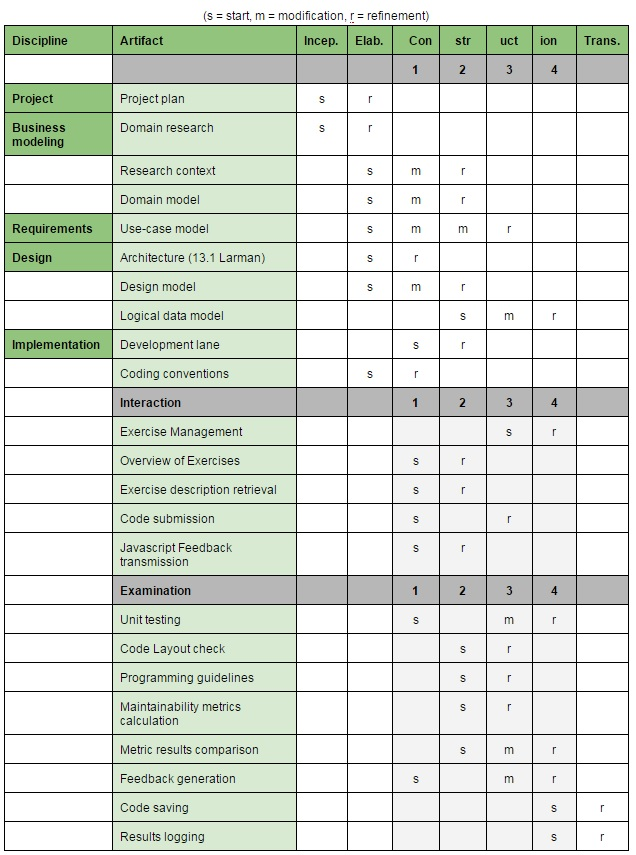
\includegraphics[scale=0.8]{iterations}
\newline
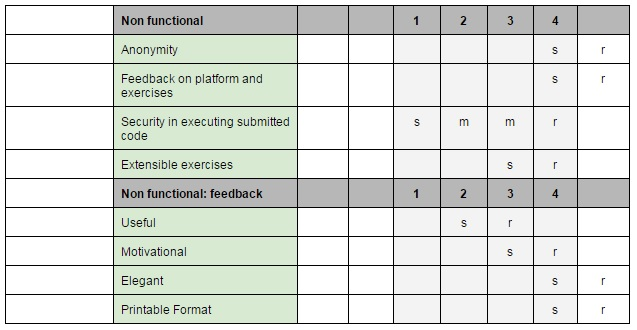
\includegraphics[scale=0.8]{iterations2}

\subsection{Evaluate project planning }

In order to keep the progress manageable, the following planning activities are
scheduled, to ensure enduring focus and facilitate possible alterations to the
planning. Missing specifics can be added as well during these activities. These
activities will be added to the agenda of the regular meetings:

\begin{tabular}{ l | p{3 cm} }
  \hline			
  Activity & Scheduled \\ \hline \hline
  Specify iteration activities (see 6.3) & 03-11-2014 \\ \hline
  Scheduling contact moments stakeholders &  27-10-2014 \newline 17-11-2014 \newline 15-12-2014 \newline 26-01-2015 \\ \hline
  Evaluate progress towards final product & 01-12-2014 \newline 12-01-2015 \\ \hline
  Evaluate meeting schedule for the remainder of the project &  19-01-2015 \\ \hline
  \hline  
\end{tabular}
\newline\newline
These dates are directives. Actual meeting moments with Stakeholders will be determined by mutal agreement. (At each
meeting, the upcoming meeting will be scheduled)

\end{document}
